\newpage
\section{Use cases}

In normal use, three types of actors can interact with the system:

\begin{itemize}
    \item \textbf{Developers} are the people that use the system to store and retrieve files. They are authenticated and authorized by the system.
    \item \textbf{Repo administrator} is the people or external system who defines the repositories and the authorizations
    \item \textbf{System administrator} is someone managing the system and its resources. He is owner of the system and defines the system configuration. He maintains and deploy the system.
\end{itemize}

\paragraph{}
Additionally, any non authenticated user is considered harmful and all interactions must be rejected.

\paragraph{}
The figure \ref{fig:use_cases} shows the use cases of these actors of the system. 

\begin{figure}[h]
    \centering
    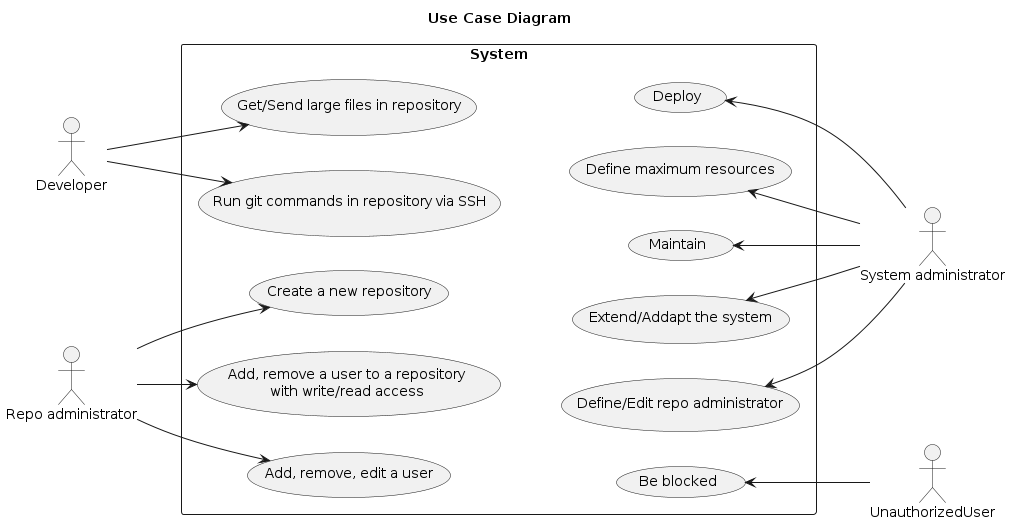
\includegraphics[width=\textwidth]{design/diagrams/use_cases.png}
    \caption{Use cases}
    \label{fig:use_cases}
\end{figure}

